\chapter{Truth} \label{truth}

Suppose that you have been trying and trying to prove a sequent, say
$\phi\vdash\psi$.  Suppose that you've spent ten hours trying to prove
it, and nothing seems to be working.  At what point would you be
justified in concluding that this sequent actually {\it cannot} be
proven --- not that it just needs a greater genius than you, but that
it is literally impossible to use the rules to derive $\psi$ from
$\phi$?

The short answer is that a failure to prove something never justifies
the conclusion that the thing cannot be proven.  It doesn't matter how
smart you are.  You could be the smartest person that ever lived, and
still, your failure to prove something is not a proof that it's
unprovable.  For example, for hundreds of years, the smartest
mathematicians in the world tried to prove a result called ``Fermat's
last theorem.''  After awhile, a lot of people started to think: the
reason these mathematicians have failed to prove it is because it must
be false!  And yet, it turns out that it is true.  In 1995, the very
patient Andrew Wiles revealed that he had a proof, which if
transcribed into our notation, would be well over a million lines
long.

The lesson is, if you want to show that something isn't provable, then
you need a different kind of evidence than your --- or anyone else's
--- failure to prove it.

One of the most amazing feats of formal logic has been in explaining
how one can prove that something cannot be proven.  In this chapter,
we explain logicians' method in the special case of propositional
logic.  It turns out that for propositional logic, it's trivially easy
to determine whether or not something can be proven.  The trick is to
find a simple, {\it detectable} feature that an argument has if it's
provable, and that an argument doesn't have if it's not provable.  For
propositional logic, the relevant feature is \emph{truth
  preservation}.  That feature only becomes detectable when we define
``truth'' in a simple mathematical way.

\section{Truth tables}

We begin with a metaphor.  Imagine that the atomic sentences
$P,Q,R,\dots $ are simple reports about contingent states of affairs.
So, for example, $P$ could be the statement, ``it rained in Princeton
on December 7, 1941''.  But remember that logic doesn't care at all
about what actually is true or false; so, for us, the symbol $P$ is
not, in itself, a true claim, or a false claim.  It only represents
the kind of statement that could be true, or could be false.

Given this picture, the state of the entire universe would be
specified by determining whether each atomic sentence $P,Q,R,\dots $
is true or false.  You could imagine that at creation, God said, ``let
$P$ be true, let $R$ be false, etc.''.  We can write all of these
possible combinations of truth values in a neat table like this:
\[ \begin{array}{c@{\, }c@{\, }c}
     P & Q & R \\
     \hline 1 & 1 & 1 \\
     1 & 1 & 0 \\
     1 & 0 & 1 \\
     1 & 0 & 0 \\
     0 & 1 & 1 \\
     0 & 1 & 0 \\
     0 & 0 & 1 \\
     0 & 0 & 0 \end{array} \] Here we have used $1$ for true, and $0$
for false -- merely as a notational convenience.  Since there are three atomic sentences, there are eight possible configurations of truth values.  The convention we've adopted is for the leftmost sentence (here $P$) to have four $1$s, and then four $0$s; then the next sentence alternates truth-values twice as quickly, etc. That pattern ensures that we pick up all possible combinations of truth values.

The idea behind truth-functional (aka Boolean) logic is that once God
chooses whether each atomic sentence is true or false, then all his
truth-making work is done -- because the truth-value of the atomic
sentences completely determines the truth-value of any complex
sentence.  For example, once God says that $P$ is true, then it
automatically follows that $\neg P$ is false.  In other words, we
should have the following relation between the truth-value of $P$ and
the truth-value of $\neg P$.
\[ \begin{array}{c | c@{}c}
     P & \neg & P \\ \hline
         1 & \mathbf{0} & 1 \\
     0 & \mathbf{1} & 0 \end{array} \]
We'll call this the \emph{truth-table} for the negation connective.
Thus, negation is simply the
Boolean ``not'' that flips $1$ and $0$.  In fact, the truth-table for
negation is applicable to any negated sentence, not just a negated
atomic sentence.  Thus, we rewrite the previous table as:
\[ \begin{array}{c | c@{}c}
     \phi & \neg & \phi \\ \hline
         1 & \mathbf{0} & 1 \\
     0 & \mathbf{1} & 0 \end{array} \]
We can already get a taste now of how to compute truth values for more
complex sentences.  Consider, for example, the sentence $\neg\neg P$.
\[ \begin{array}{c | c@{}c@{}c } P & \neg &\neg & P \\ \hline
     1 & \mathbf{1}  & 0 & 1 \\
     0 & \mathbf{0} & 1 & 0 \end{array} \] Here we use the truth-value
 of $P$ to compute the truth-value of $\neg P$; and then we use the truth-value of $\neg P$ to compute the truth-value of $\neg \neg P$.  The \emph{\gls{main column}} (in bold font) is the column that is filled in {\it last} as we go through the process.  It represents the truth value that the sentence $\neg\neg P$ has in each different situation.

Now we've got to decide on how to compute truth values for
conjunctions, disjunctions, and conditionals.  The case of conjunction
is the most clear: a conjunction is true just in case both conjuncts are
  true. In particular, for $P\wedge Q$ to be true, both
$P$ and $Q$ must be true.  If one or both of $P$ and $Q$ is false,
then $P\wedge Q$ is false. That yields the following table.
\[ \begin{array}{ c@{\, }c | c@{\, }c@{\, }c}
P & Q &  P & \wedge & Q  \\
\hline 
1 & 1 &  1 & \mathbf{1} & 1  \\
1 & 0 &  1 & \mathbf{0} & 0  \\
0 & 1 &  0 & \mathbf{0} & 1  \\
0 & 0 &  0 & \mathbf{0} & 0  \\
   \end{array} \]
 A similarly simple rule allows us to
 compute the truth value of a disjunction: a disjunction is true just in case at least one of its
 disjuncts is true. This leads to the following
 truth-table.
\[ \begin{array}{ c@{\, }c | c@{\, }c@{\, }c}
P & Q &  P & \vee & Q  \\
\hline 
1 & 1 &  1 & \mathbf{1} & 1  \\
1 & 0 &  1 & \mathbf{1} & 0  \\
0 & 1 &  0 & \mathbf{1} & 1  \\
0 & 0 &  0 & \mathbf{0} & 0  \\
   \end{array} \] 
 Now, if you put your critical thinking cap on, you might conclude that this disjunction rule is {\it
   bad}, because a disjunction shouldn't be true when {\it both}
 disjuncts are true.  We think that's a reasonable objection, and it
 would be good, at some point, to reflect further on other possible
 options for giving a precise, formal representation of the logical
 notion of disjunction.  But for now, please recall that we are
 building an {\it idealized model} of human logic, which means that
 there may be some mismatch between the model and our intuitions.

The truth-value of a complex sentence $\phi$ can be calculated by
working from the inside out.  One begins by copying the truth values
of atomic sentences $P,Q,R,\dots$ in each row of the truth-table over
to columns under places where those atomic sentences occur in $\phi$.
Then those truth values are used in combination with the tables for
$\neg ,\vee ,\wedge$ to compute truth-values of the more complex
sub-formulas of $\phi$, and so on, until we reach the \emph{main
  connective} of $\phi$, which is the last connective that is inserted
in the construction of $\phi$.  For the specific case where $\phi$ is
the sentence $\neg P\vee (Q\wedge R)$, we computed the full table below.
\[ \begin{array}{ c@{\, }c@{\, }c | c@{ }c@{\, }@{\, }c@{\, }c@{ }c@{\, }@{\, }c@{\, }@{\, }c@{\, }@{ }c@{ }@{}c@{}@{ }c}
     P & Q & R   & \neg  & P & \vee & ( & Q & \wedge  & R & ) & \\
\hline 
1 & 1 & 1   & 0 & 1 & \mathbf{1} &  & 1 & 1 & 1 &  & \\
1 & 1 & 0   & 0 & 1 & \mathbf{0} &  & 1 & 0 & 0 &  & \\
1 & 0 & 1   & 0 & 1 & \mathbf{0} &  & 0 & 0 & 1 &  & \\
1 & 0 & 0   & 0 & 1 & \mathbf{0} &  & 0 & 0 & 0 &  & \\
0 & 1 & 1   & 1 & 0 & \mathbf{1} &  & 1 & 1 & 1 &  & \\
0 & 1 & 0   & 1 & 0 & \mathbf{1} &  & 1 & 0 & 0 &  & \\
0 & 0 & 1   & 1 & 0 & \mathbf{1} &  & 0 & 0 & 1 &  & \\
0 & 0 & 0   & 1 & 0 & \mathbf{1} &  & 0 & 0 & 0 &  & \\
   \end{array} \]
 Let's call this table the \emph{truth table} for the sentence
 $\neg P\vee (Q\wedge R)$.  To this point, we have been casual with our understanding of what
 counts as a sentence of propositional logic.  However, in order to
 compute truth tables, it's important to note that any legitimate
 sentence is built up in a unique way from propositional constants such
 as $P,Q$ and $R$.  As a result, if a sentence $\phi$ is not itself one
 of these propositional constants, then there is one connective ---
 the so-called \emph{main connective} --- that is
 the last one in its construction.  (For more details, see page
 \pageref{formation}.)  
 The main connective of $\neg P\vee (Q\wedge R)$ is
 $\vee$, and we have highlighted the column under that connective in the
 truth table.  The values in this \emph{main column} give the status
 of the sentence $\neg P\vee (Q\wedge R)$ in all the different
 possible situations.

\begin{exercise} Write the truth table for $P\wedge\neg P$.  How do
  you interpret the significance of the result? \end{exercise}



You can now compute the truth values for any complex sentence built
with negation, conjunction, and disjunction.  But what about sentences
built with the conditional symbol? The table is as follows:
\[ \begin{array}{ c@{\, }c | c@{\, }c@{\, }@{\, }c@{ }@{ }c@{ }@{ }c}
P & Q &  P & \to  & Q & \\
\hline 
1 & 1  & 1 & \mathbf{1} & 1 & \\
1 & 0  & 1 & \mathbf{0} & 0 & \\
0 & 1  & 0 & \mathbf{1} & 1 & \\
0 & 0  & 0 & \mathbf{1} & 0 & \\
   \end{array} \]
 You'll need to accept this truth-table, and use it to solve
 problems.  But we want to be upfront about the fact that this truth
 table does not simply and obviously capture the true meaning of
 ``if\dots then.''  For example, ``The moon is made of green cheese'' is
 false, and ``Caesar crossed the Rubicon'' is true, hence the table
 suggests that it's true that: ``If the moon is made of green cheese
 then Caesar crossed the Rubicon.''  That seems rather odd.  And the
 oddness only increases if you cook up examples for rows one and
 four.  The only row that seems obviously correct is the second row.
 
 At this point, symbolic logic comes to a substantial philosophical
 crossroads.  In short, {\it there is no truth-table that adequately
   captures the nuance of the ``if \dots then \dots '' connective in
   natural languages}.  In the twentieth century, philosophers spent
 {\it a lot} of time worrying about this nasty little connective
 $\to$, and they came up with many more or less interesting
 proposals.\footnote{You can learn more about these issues in a course
   or book about \emph{philosophical logic}.  For example, ``relevance
   logic'' was invented precisely to avoid the paradoxes of material
   implication. See p.\ \pageref{relevant} for references.} Meanwhile,
 there's a strong case to be made that this truth-table -- and the
 corresponding rules MP and CP -- are the de facto standard used in
 mathematics and the sciences.

For our current agenda, the important fact is simply that the truth
table for $\to$ matches with the inference rules CP and MP in a
precise sense that we will explain soon -- when we talk about the
soundness and completeness theorems.  What that means is that if you
want to change the truth table for $\to$, then you need different
inference rules.  And if you want different inference rules for $\to$,
then you need a different truth table.

Once we've agreed upon the truth-table for the conditional, we can
compute the truth-table for the biconditional.
\[ \begin{array}{c@{\, }c | c@{\, }c@{\, }c@{ }c c}
P & Q &   P & \leftrightarrow & Q & \\
\hline 
1 & 1 &   1 & \mathbf{1} & 1 & \\
1 & 0 &   1 & \mathbf{0} & 0 & \\
0 & 1 &   0 & \mathbf{0} & 1 & \\
0 & 0 &   0 & \mathbf{1} & 0 & \end{array} \]
In other words, a biconditional $P\lra Q$ is true just in case $P$ and
$Q$ have the same truth-value.

\begin{exercise} Compute the truth-table for $\neg P\lra \neg Q$.  How
  do you interpret the significance of the result? \end{exercise}

\section{Truth in the service of proof}

What can you {\it do} with these truth tables?  What's their cash
value?  Writing out a truth table is not a particularly challenging
exercise --- and so it's not a good way to try to build mental muscle.
The true utility of truth tables (for us, in this context) is that
they can show us what can and cannot be proven.

As you surely have experienced, the process of discovering a proof
involves genuine strategic thinking.  Especially for the longer and
more difficult proofs, you have to choose appropriate intermediate
goals.  But how do you decide on those intermediate goals?  How do you
know which intermediate goals are attainable, and how do you know
which intermediate goals will get you closer to the destination?
Mistakes here can be costly.  If you choose an intermediate goal that
cannot be proven, then you might waste an enormous amount of time
trying to prove it.  Conversely, if you choose an intermediate goal
that is too weak to obtain the conclusion, then you'll be trapped in a
dead end.

To understand how truth-tables can be used in the service of proof,
you need to know two facts.  We will demonstrate these facts in
Chapter \ref{meta}; but at present, you'll have to take our word for
it.  First, a bit of terminology.
\begin{defn} Let $\phi _1,\dots ,\phi _n$ and $\psi$ be sentences.
  Let's say that the argument from $\phi _1,\dots ,\phi _n$ to $\psi$
  is \emph{truth-preserving} just in case in the truth table for all
  $n+1$ sentences, in any row where each of $\phi _1,\dots ,\phi _n$
  is assigned $1$, the sentence $\psi$ is also assigned
  $1$. \end{defn}
Here now is the first of the two facts that you need to know:

\begin{sothm} If $\phi _1,\dots ,\phi _n\vdash \psi$, then
  the argument from $\phi _1,\dots ,\phi _n$ to $\psi$ is
  truth-preserving. \end{sothm}

The contrapositive of the \gls{soundness theorem} says that if there's
any case where $\phi _1,\dots ,\phi _n$ are true and $\psi$ is false,
then $\psi$ can {\it not} be proven from $\phi _1,\dots ,\phi _n$.
The upshot is:
\begin{quote} If there is a truth-table row in which
  $\phi _1,\dots ,\phi _n$ are true, and $\psi$ is false, then there
  is no proof from $\phi _1,\dots ,\phi _n$ to $\psi$. \end{quote}
Such a truth-table row is known as a \emph{\gls{counterexample}} to
the validity of the argument.

%% affirming the consequent

To take a simple example, consider the argument $P\to Q,Q\:\vdash P$,
which you know intuitively to be invalid --- indeed, it's the
notorious fallacy of affirming the consequent.  The truth table for
this argument looks like this:
\[ \begin{array}{ c@{\, }c | c@{ }c@{ }c@{ }c@{ }c | c | c p{4cm} }
P & Q &  & P & \rightarrow & Q &  & Q & P\\
\cline{1-9} 
1 & 1 &  & 1 & \mathbf{1} & 1 &  & \mathbf{1} & \mathbf{1}\\
1 & 0 &  & 1 & \mathbf{0} & 0 &  & \mathbf{0} & \mathbf{1}\\
0 & 1 &  & 0 & \mathbf{1} & 1 &  & \mathbf{1} & \mathbf{0} &
                                                             $\Longleftarrow$
                                                             counterexample \\
0 & 0 &  & 0 & \mathbf{1} & 0 &  & \mathbf{0} & \mathbf{0}\\
   \end{array} \]
In the first two rows of the truth table, the conclusion $P$ is true
-- and so those rows don't provide any interesting information about
the argument.  The third row, however, raises a red flag: here the two
premises $P\to Q$ and $Q$ are both true, and the conclusion $P$ is
false.  That's a counterexample.  Hence, by the soundness theorem,
there is no proof from $P\to Q$ and $Q$ to $P$.

In the special case of an argument with no premises, i.e.\ where the
conclusion $\psi$ is simply asserted, the truth-preservation condition
says that: whenever all the premises are true (which is always, since
there are none of them), the conclusion $\psi$ is true.  Hence, the
soundness theorem says that the sequent $\vdash\phi$ is provable only
if $\phi$ is always true, in every row of its truth table.
Contrapositively, if $\phi$ is ever false, then the sequent
$\vdash\phi$ cannot be proven.  For example, and unsurprisingly, the
sequent $\vdash P$ cannot be proven.

Let's see now how the soundness theorem can prevent you from choosing
a bad proof strategy.  Suppose that you've been asked to prove
$\vdash (P\to Q)\vee (Q\to P)$. Since the conclusion is a disjunction,
you might reasonably think that a good strategy would be to try to
prove $\vdash P\to Q$, then to infer the conclusion by means of
$\vee$I.  However, $P\to Q$ is {\it not} a tautology; which means that
$\vdash P\to Q$ cannot be proven.  Hence, that would be a disastrously
bad strategy.

So, the soundness theorem provides a method for proving that something
cannot be proven.  We already know one way of proving that something
can be proven: by producing a proof of it.  Amazingly, though, there
is another way of proving that something can be proven.  The
completeness theorem tells us that if a sequent is truth-preserving,
then it can in fact be proven.
\begin{description}
\item[Completeness theorem] If the argument from $\phi _1,\dots ,\phi _n$ to
  $\psi$ is truth-preserving, then
  $\phi _1,\dots ,\phi _n\vdash \psi$.
\end{description}
In the special case of $n=0$, it follows that if $\phi$ is a
tautology, then $\vdash \phi$.  For example, it's easy to see that
$P\vee \neg P$ is a tautology: if $P$ is true, then $P\vee \neg P$ is
true; and if $P$ is false, then $\neg P$ is true, and $P\vee\neg P$ is
true.  Similarly, a quick truth-table test shows that Pierce's
proposition is a tautology, and hence can be proven.
\[ \begin{array}{@{ }c@{ }@{ }c | c@{ }@{}c@{}@{}c@{}@{ }c@{ }@{ }c@{ }@{ }c@{ }@{}c@{}@{ }c@{ }@{ }c@{ }@{}c@{}@{ }c@{ }@{ }c@{ }@{ }c}
P & Q &  & ( & ( & P & \rightarrow & Q & ) & \rightarrow & P & ) & \rightarrow & P & \\
\hline 
1 & 1 &  &  &  & 1 & 1 & 1 &  & 1 & 1 &  & \mathbf{1} & 1 & \\
1 & 0 &  &  &  & 1 & 0 & 0 &  & 1 & 1 &  & \mathbf{1} & 1 & \\
0 & 1 &  &  &  & 0 & 1 & 1 &  & 0 & 0 &  & \mathbf{1} & 0 & \\
0 & 0 &  &  &  & 0 & 1 & 0 &  & 0 & 0 &  & \mathbf{1} & 0 & \\
   \end{array} \]


 \begin{exercise} Write truth-tables for $\neg P\vee Q$ and $P\to Q$,
   and say whether either one implies the other. \end{exercise}
\begin{exercise} Show that $P$ cannot be derived from $P\lra
  Q$. \end{exercise}
\begin{exercise} Explain why $P\wedge\neg P\vdash Q$ is truth-preserving.
\end{exercise}
 

% We won't prove the soundness theorem until Chapter \ref{meta}, but we
% can already get a feeling for why it's true.  Let's think, in
% particular, about some of the more surprising inference rules, and
% about some of the more surprising truth tables.  Recall first your
% surprise when you realized that the rule of conditional proof did not
% require you to use the assumption.  Thus, one gets the strange result
% that the following sort of argument is valid:
% \[ \begin{array}{l l >{$}p{1.75cm}<{$} p{2cm}}
%      1 & (1) & Q & A \\
%      2 & (2) & P & A \\
%      1 & (3) & P\to Q & 2,1 CP \end{array} \]
% Why, from a truth-preservation point of view, is this move acceptable?
% In short, the truth table for $P\to Q$ says that it's true whenever
% $Q$ is true, no matter the truth value of $P$.  Now, the move from 1
% to 3 in the argument above essentially says that {\it if} it has
% already been established that the argument $\Gamma\vdash Q$ is good,
% {\it then} the argument $\Gamma\vdash P\to Q$ is also good.  To be
% more precise, we'll say that an argument is {\it good} just in case
% it's truth preserving, i.e.\ whenever its premises are good, so is its
% conclusion.  But now if $\Gamma\vdash Q$ is good, and if all the
% sentences in $\Gamma$ are true then $Q$ is true.  Hence by the truth
% tables, $P\to Q$ is true.  Therefore, whenever $\Gamma$ is true, so is
% $P\to Q$, and the argument $\Gamma\vdash P\to Q$ is good.

% Similarly, you might have felt shocked and betrayed when you learned
% that any sentence $Q$ can be derived from a contradiction
% $P\wedge\neg P$.  However, in terms of truth-preservation, that
% argument is perfectly good: since $P\wedge\neg P$ is never true, it is
% trivially the case that whenever $P\wedge\neg P$ is true, so also is
% $Q$.  In other words, the argument $P\wedge\neg P\vdash Q$ cannot
% possibly fail to be truth-preserving, because there is never a
% scenario in which its premises are true.

\section{Short cuts}

The correspondence between proofs and truth tables gives a
handy way to classify sentences.  We define three mutually
exclusive and exhaustive classes of sentences:
\begin{itemize}
\item A sentence is an \emph{\gls{inconsistency}} just in case its
  truth-value is always $0$.  (Here ``always'' means ``on every row of
  its truth table, under the main connective''.)
\item A sentence is a \emph{\gls{tautology}} just in case its
  truth-value is always $1$.  By soundness and completeness, $\phi$ is
  a tautology just in case $\vdash\phi$.
\item A sentence is a \emph{\gls{contingency}} just in case its
  truth-value is sometimes $0$ and sometimes $1$.
\end{itemize}
You already know paradigm examples of each kind of sentence:
$P\vee\neg P$ is a tautology, $P\to P$ is a tautology, $P\wedge\neg P$
is an inconsistency, $P$ is a contingency, and $P\vee Q$ is a
contingency.

We can also give precise definitions for logical relations between
sentences.
\begin{itemize}
\item Two sentences $\phi$ and $\psi$ are \emph{logically equivalent} just in
  case $\phi$ and $\psi$ have the same value in all rows of their
  common truth table.  By soundness and completeness, $\phi$ and
  $\psi$ are logically equivalent just in case $\vdash \phi\lra\psi$.
\item A set $\Gamma$ of sentences is \emph{consistent} just in case
  there is at least one row in their common truth table in which all
  sentences in $\Gamma$ have value $1$.  If $\Gamma$ is not
  consistent, then we say it is \emph{inconsistent}.    
\end{itemize}

We previously used the word \emph{inter-derivable} for two sentences
$\phi$ and $\psi$ when there are proofs $\phi\vdash\psi$ and
$\psi\vdash\phi$, which we wrote as $\phi\dashv\vdash\psi$.  Clearly,
$\phi\dashv\vdash\psi$ just in case $\vdash\phi\lra\psi$, and it will
be convenient sometimes to write $\phi\equiv\psi$ as shorthand for
this relation of inter-derivability.  The soundness and completeness
theorems guarantee that $\phi$ and $\psi$ are inter-derivable just in
case $\phi$ and $\psi$ are logically equivalent.  (On page
\pageref{equivs}, we've given a list of several pairs of
inter-derivable -- hence logically equivalent -- sentences.)

%% TO DO: explain that interderivability is an equivalence relation

 
%% all contradictions are logically equivalent
%% an inconsistency implies everything else

%% exercise: remember those exercises I had on the exams, where I
%% asked if something was a fragment of a correctly written proof

\begin{example} We will prove that if $\phi\dashv\vdash\psi$ then
  $\vdash\phi\lra\psi$.  Take note: our proof here is {\it not} a
  single formal proof with dependency numbers, etc.  Instead, it is a
  meta-theoretic argument about the existence of certain formal
  proofs.

  We assume then that $\phi\dashv\vdash\psi$.  This says that there
  are two formal proofs, one proof of $\phi\vdash\psi$ and one proof
  of $\psi\vdash\phi$.  By the conditional proof rule, these two
  proofs can be extended to proofs of $\vdash\phi\to\psi$ and of
  $\vdash\psi\to\phi$.  Then those two proofs can be concatenated, and
  combined with an instance of conjunction introduction to give
  $\vdash(\phi\to\psi)\wedge (\psi\to \phi)$, and an instance of
  biconditional introduction to give $\vdash
  \phi\lra\psi$. \end{example}

\begin{exercise} Show that if $\vdash\phi\lra\psi$ then
  $\phi\dashv\vdash\psi$. \end{exercise}
 
Truth tables are easy \dots and also inefficient and potentially
mind-numbing.  After you've done a dozen of them, you realize that you
won't learn anything by doing more.  It's time either to find a
computer program to do them for you, or better, discover some rules of
thumb to find the relevant lines of a truth table without writing out
the whole thing.  This section is highly pragmatic and
non-theoretical.  The one and only goal is to provide you with some
rules of thumb for finding relevant truth-table rows.

Suppose, for example, that you want to know whether the sequent
\[ P\vee Q,\,R\wedge \neg Q\:\vdash\:R\to \neg P ,\] can be proven or
not.  If you write up a full truth-table, you'll need eight rows.  But
notice that the only potential counterexamples are the rows where the
conclusion $R\to \neg P$ is false, hence rows where $R$ and $P$ are
true.  A quick inspection of the premises shows that the first is true
whenever $P$ is true; and if $R$ is true, then the second is true when
$\neg Q$ is true.  So there you have it: the following row of the
truth table provides a counterexample to the validity of this
argument.
\[ \begin{array}{ c@{\, }c@{\, }c | c@{\, }c@{\, }c c@{\, }c@{\, }c@{ }c c@{\,
     }c@{\, }c@{ }c }
P & Q & R & P & \vee & Q & R & \wedge & \neg & Q & R & \to & \neg &
                                                                    P
     \\
     \hline
1 & 0 & 1 & 1 & \mathbf{1} &   0  & 1 & \mathbf{1}      & 1    & 0 & 1 & \mathbf{0}   & 0 & 1 \end{array} \]
Each row of a truth table corresponds to an assignment of $0$s and
$1$s to the atomic sentences.  We call such an assignment a
\emph{valuation}, and we can write it in functional form like this: $v(P)=1$, $v(Q)=0$, and
$v(R)=1$.  The valuation $v$ here makes the premises of the argument
true, and the conclusion false.  Hence, the argument fails to be truth
preserving, and the conclusion cannot be proven from the premises.

This first example shows that when the conclusion of an argument is a
conditional, then you can immediately narrow focus to the lines where
its antecedent is true, and its consequent is false.  The same kind of
rule of thumb applies to a disjunctive conclusion: the only relevant
lines are those where both disjuncts are false.  Unfortunately, the
situation is worse when the conclusion is a conjunction, for there are
three different ways that a conjunction can be false.

Consider now a different example: you want to know whether the sequent
$P\wedge Q,\neg Q\vee R\vdash R$ can be proven.  In this case, the
conclusion is an atomic sentence $R$; so you can focus only on those
rows where $R$ is false.  Among those rows where $R$ is false, the
first premise is true only if both $P$ and $Q$ are true.  But that is
all the information we need, for if $Q$ is true and $R$ is false, then
the second premise is false.  In other words, there is no row in which
the premises are true and the conclusion is false.  This argument is
valid, and the sequent can be proven.

What we just did is a lot like playing a game of Sudoku.  The key to
doing it properly is not to make guesses --- you only assign a truth
value to a sentence when you are forced to buy the supposition that the
conclusion is false and the premises are true.  Here, in fact, is how
we are arguing:
\[ \begin{array}{p{10cm}}
     Suppose that the argument from $\phi _1$ and $\phi _2$ to $\psi$
     is invalid. \\
     There is a row in the truth table where $\phi _1$ and $\phi _2$
     are true, but $\psi$ is false. \\
     If $\psi$ is false, then \dots \\
     If $\phi _1$ and $\phi _2$ are true, then \dots \\
     {[}some contradiction{]} \\
     Therefore, the argument from $\phi _1$ and $\phi _2$ to $\psi$ is
     valid. \end{array} \]
To draw such a conclusion, you've got to be careful about the steps
``If $\psi$ is false, then \dots '' and ``If $\phi _1$ and $\phi _2$
are true then \dots ''.

In some cases, you simply won't be forced by the suppositions to
assign particular truth-values; instead, you'll have options.  Then
you have to search systematically through the options to see if there
is a counterexample to the argument.  Consider one more example: you
want to know if the argument $(P\wedge Q)\to R\vdash P\to (Q\wedge R)$
is valid.  If the conclusion is false, then $P$ is true and
$Q\wedge R$ is false.  But sadly, there are three ways that
$Q\wedge R$ can be false.  If the premise is true, then sadly we can't
say much either.  It could be that $R$ is true, or it could be that
$P\wedge Q$ is false, and there are three ways that it could be false.
At this stage, we can just try out various values for $Q$ and $R$.
Noticing that the premise is true whenever $R$ is true, we can check
if the conclusion can be made false in that case.  Indeed, if $Q$ is
false, then $Q\wedge R$ is false, and the conclusion is false.  So
there we have it: if $P$ and $R$ are true, and $Q$ is false, then the
premise is true and the conclusion is false.  This argument is
invalid, and the sequent cannot be proven.

This kind of argumentation about truth-preservation can sometimes
shade into a formal proof, where the only thing that's missing are the
dependency numbers, and the explicit citation of inference rules.
Consider, for example, an argument that if the premise
$P\wedge (Q\vee R)$ is true, then so is the conclusion
$(P\wedge Q)\vee (P\wedge R)$.
\[ \begin{array}{p{11cm}}
     $(1)$ Suppose that $P\wedge (Q\vee R)$ is true.  \\
     $(2)$ Then both $P$ and $Q\vee R$ are true. \\
     $(3)$ Since $Q\vee R$ is true, either $Q$ or $R$ is true. \\
     $(4)$ If $Q$ is true, then $P\wedge Q$ is true, hence $(P\wedge
     Q)\vee (P\wedge R)$ is true.  \\
     $(5)$ If $R$ is true, then $P\wedge R$ is true, hence $(P\wedge
     Q)\vee (P\wedge R)$ is true.  \\
     $(6)$ In either case, $(P\wedge Q)\vee (P\wedge R)$ is
     true.  \end{array} \]
Here line $2$ is justified by conjunction elimination.  Line 3 looks a
bit like disjunction elimination, but in fact it's just the statement
of the definition of the truth table for $\vee$.  The transition from
line 1 to line $2$ also involves a tacit invocation of the truth table
for $\wedge$.  Lines 4 and 5 each result from one step
of conjunction introduction, and one step of disjunction
introduction.  Line 6 results from disjunction elimination.

Let's write the first bit of this argument again, bringing it even
closer in line with complete formalization.
\[ \begin{array}{l l >{$}p{6cm}<{$} p{3cm}}
     1 & (1) & v(P\wedge (Q\vee R))=1 & A \\
     1 & (2) & v(P)=1 \;\text{and}\; v(Q\vee R)=1 & def $\wedge$ \\
     1 & (3) & v(Q\vee R)=1 & 2 and elim \\
     1 & (4) & \text{Either}\;v(Q)=1\;\text{or}\;v(R)=1 & def $\vee$
     \\
     5 & (5) & v(Q)=1 & A \\
     1 & (6) & v(P)=1 & 2 and elim \\
     1,5 & (7) & v(P)=1\;\text{and}\;v(Q)=1 & 5,6 and intro \\
     1,5 & (8) & v(P\wedge Q)=1 & def $\wedge$  \\
     1,5 & (9) & v((P\wedge Q)\vee (P\wedge R))=1 & def $\vee$ 
               \end{array} \]
We could continue here by deriving $v((P\wedge Q)\vee (P\wedge R))=1$
from the assumption that $v(R)=1$.  Then we could use $\vee$
elimination to eliminate dependency on the assumptions $v(Q)=1$ and
$v(R)=1$.  The end result would be a proof of the sequent
\[ v(P\wedge (Q\vee R))=1 \;\vdash\; v((P\wedge Q)\vee (P\wedge R))=1 .\]
To argue in such an explicit fashion can have the advantage of
convincing you that you really are using the rules of logic.  However,
there are also disadvantages to arguing completely explicitly.  One
disadvantage is simple inefficiency.  If your goal is to convince
somebody else, then you only need to say as much as is necessary to
convince them that a formal proof exists.

Notice also that the conclusion we really want isn't the
sequent:
\begin{equation} v(P\wedge (Q\vee R))=1 \; \vdash \; v((P\wedge Q)\vee (P\wedge
  R))=1 , \tag{$\ast$} \end{equation} 
it's the general claim:
\[ \text{For every $v$},\:\bigl[ v(P\wedge (Q\vee R))=1 \; \vdash \;
  v((P\wedge Q)\vee (P\wedge R))=1 \bigr] .\] While it's intuitively
clear that we have proved the general claim, we don't yet have an
inference rule that will let us get from sequent ($\ast$) to the
general claim.  To do that, we need to be able to talk about ``all
valuations,'' i.e.\ we need to be able to quantify over valuations.
That's the subject of predicate logic, which we take up in the next
chapter.
                                     
\begin{exercises} Provide counterexamples to the following invalid
  argument forms.
  \begin{enumerate}
  \item $P\to Q,Q\:\vdash\: P$  
  \item $P\to R\:\vdash\: (P\vee Q)\to R$
  \item $P\to R\:\vdash\: P\to (Q\wedge R)$
  \item $P\to (Q\to R)\vdash\: (P\to Q)\to R$  
  \end{enumerate}
\end{exercises}

\begin{exercises} Classify each of the following sentences as
  tautology, inconsistency, or contingency.
  \begin{enumerate}
  \item $(P\to Q)\vee (Q\to R)$
\item $(P\to Q)\vee (P\to R)$
  \item $(P\wedge Q)\vee (P\wedge \neg Q)\vee (\neg P\wedge Q)$  
  \item $(P\to \neg P)\to P$
  \item $P\to (\neg P\to P)$
  \end{enumerate}
\end{exercises}

\begin{exercises} Show that the following pairs of sentences are
  logically equivalent (i.e.\ always have the same truth-value):
  \begin{enumerate}
  \item $P\:\equiv\:\neg P\to P$  
  \item $Q\:\equiv\: P\lra (P\lra Q)$
  \item $P\lra R\:\equiv\: (P\lra Q)\lra (Q\lra R)$ \end{enumerate} \end{exercises}

\begin{exercises} Are the following sequents provable?  Explain your
  answers.
  \begin{enumerate}
  \item $\vdash\: (P\to P)\to \neg P$
  \item $P\lra Q\:\vdash\: \neg P\lra \neg Q$
  \item $\vdash\:(P\lra Q)\vee (Q\lra P)$
    \item $\vdash \:(P\lra Q)\vee (P\lra R)\vee (P\lra R)$  
  \end{enumerate}
\end{exercises}

\begin{exercise} Show that the $\to$ connective is not associative.
  That is, show that $P\to (Q\to R)$ is not equivalent to
  $(P\to Q)\to R$. \end{exercise}

\begin{exercise}  Suppose that you're tutoring another student who is
  trying to prove the sequent:
  \[ P\to (Q\vee R)\:\vdash\: (P\to Q)\vee (P\to R) .\] That student
  says that he'll try first to prove $P\to Q$, and then use $\vee$
  introduction to get the result.  Do you think his strategy is good?
\end{exercise}

\begin{exercise} Suppose that the sentence $\phi$ is an inconsistency.
  What can you say about the sentence $\phi\to\psi$? \end{exercise}

\begin{exercise} Suppose that the sentence $\phi\wedge\neg\psi$ is an
  inconsistency.  Explain how you know that the sequent
  $\phi\vdash\psi$ is provable. \end{exercise}

%% \begin{exercise} Write out a semi-formal proof that Pierce's prop
%% is a tautology


\section{Propositions as Sets of Possible Worlds}

There's another way of thinking about the relation between sentences
and truth-values --- a way that philosophers use to frame many of
their discussions.  Let's think of a truth-valuation (i.e.\ a row in a
truth table) as a ``way that things could be.''  Philosophers
sometimes like to use the phrase ``possible world'' for a way that
things could be.  Now we can imagine all of these ``ways that things
could be'' to be gathered together into a single collection, a sort of
meta-universe of all possible worlds.  Imagine, for the sake of this
discussion, the point of view of an omnipotent being who might be
contemplating the question: ``which world should I create?''  As this
omnipotent being surveys all of the possible worlds, she might decide
that certain things are important to her --- e.g.\ She might decide
that She wants a world in which there are colorful flowers.  Let $P$
be shorthand for the sentence, ``there are colorful flowers.''  Then
She could decide to rule out all worlds where there are no colorful
flowers, i.e.\ all worlds in which $P$ is false, and $\neg P$ is true.
In short, She can use propositions like $P$ to pick out a
sub-collection of worlds that have a certain feature.

Although we lack the power to create worlds, we do have the power to
imagine all possible worlds, and to use propositions to differentiate
worlds from each other.  In fact, it seems that the job of science is
to figure out more and more about where we live in the space of all
possible worlds.  That is, science tries to find which propositions
are true, because each such proposition narrows down the set of
possible locations of {\it our} world in the space of all possible
worlds.

Now let's try to turn this suggestive idea into a useful tool for
reasoning.  In this section, we'll just look at the case where there
are two atomic sentences: $P$ and $Q$.  In that case, there are four
truth-valuations, and hence four possible worlds $v_1,v_2,v_3,v_4$.
(In general, if there are $n$ atomic sentences, then there are $2^n$
possible worlds, and if there are infinitely many atomic sentences,
then there is an uncountable infinity of possible worlds.)  Let's
imagine these worlds as blocks in a $4\times 4$ grid.  The top blocks
are those in which $v(P)=1$, and the left blocks are those in which
$v(Q)=1$.
%% TO DO: Go ahead and write the four valuations here to the right
\begin{figure}[h]
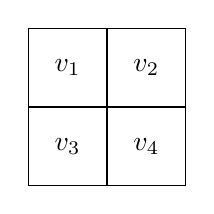
\begin{tikzpicture}[every node/.style={minimum size=1cm-\pgflinewidth, outer sep=0pt}]  
  \draw[step=1cm,color=black] (-1,-1) grid (1,1);
  \node at (-0.5,+0.5) {$v_1$};
  \node at (-0.5,-0.5) {$v_3$};
  \node at (+0.5,+0.5) {$v_2$};
  \node at (+0.5,-0.5) {$v_4$};
\end{tikzpicture}
\end{figure}

If you don't know anything at all, then all bets are off --- you could
be in any of the worlds $v_1,v_2,v_3,v_4$.  Furthermore, if you only
know a tautology, say $P\vee\neg P$, then you could be in any world.
That's what it means to say that tautologies are empty or contentless:
they don't rule out any possibilities.  If, in contrast, you know that
$P$, then you know that you're not in one of the bottom two worlds.
Hence, the proposition $P$ can be represented by graying the bottom
row.
\begin{figure}[h]
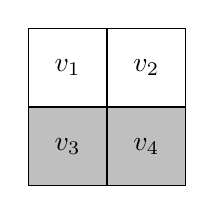
\begin{tikzpicture}[every node/.style={minimum size=1cm-\pgflinewidth, outer sep=0pt}]
    \draw[step=1cm,color=black] (0,-1) grid (2,1);
    \node[fill=gray!50] at (+0.5,-0.5) {$v_3$};
    \node[fill=gray!50] at (+1.5,-0.5) {$v_4$};
    \node at (+0.5,+0.5) {$v_1$};
    \node at (+1.5,+0.5) {$v_2$};
\end{tikzpicture}
  \caption{The proposition $P$ rules out possibilities $v_3$ and $v_4$.}
\end{figure}
Similarly, the proposition $Q$ can be represented by graying out the
column on the right; the proposition $\neg P$ can be represented by
graying out the top row; and the proposition $\neg Q$ can be
represented by graying out the column on the left.

Interestingly, this visual representation indicates that there are
``missing propositions'' that are of the same logical kind as $P$ and
$Q$ --- that is, other propositions that gray out two squares.
Consider, for example, the case where the top-right and bottom-left
square are grayed out.  The corresponding proposition $\phi$ doesn't
rule out $P$, and it doesn't rule out $Q$, and it doesn't rule out
either $\neg P$ or $\neg Q$.  What it does rule out are the
cross-cases where $P$ is true and $Q$ is false; and when $P$ is false
and $Q$ is true.  In other words, $\phi$ demands that $P$ have the
same truth-value as $Q$.  We see then that the proposition $\phi$
isn't missing after all: it's the proposition $P\lra Q$.

Propositions like $P$ and $Q$ leave open more than one possibility.
The tautologies, such as $P\vee\neg P$ leave open all possibilities;
and the contradictions, such as $P\wedge\neg P$ leave open no
possibilities (i.e.\ they cannot be true).  Another interesting kind
of proposition are those maximally specific propositions that leave
open only one possibility.  In this case, there are four maximally
specific propositions, represented by
$P\wedge Q,P\wedge\neg Q,\neg P\wedge Q$, and $\neg P\wedge\neg Q$.
\begin{figure}[h]
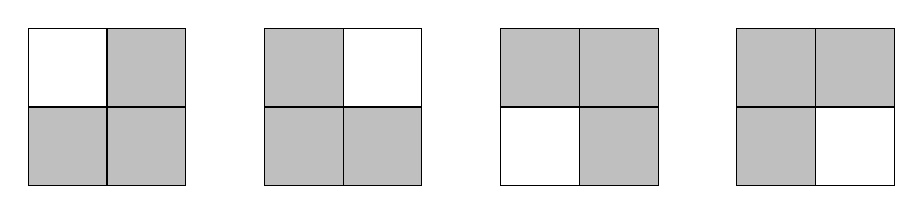
\begin{tikzpicture}[every node/.style={minimum size=1cm-\pgflinewidth, outer sep=0pt}]
    \draw[step=1cm,color=black] (-1,-1) grid (1,1);
    \node[fill=gray!50] at (-0.5,-0.5) {};
    \node[fill=gray!50] at (+0.5,+0.5) {};
    \node[fill=gray!50] at (+0.5,-0.5) {};
    \draw[step=1cm,color=black] (2,-1) grid (4,1);
    \node[fill=gray!50] at (+2.5,+0.5) {};
    \node[fill=gray!50] at (+2.5,-0.5) {};
    \node[fill=gray!50] at (+3.5,-0.5) {};
    \draw[step=1cm,color=black] (5,-1) grid (7,1);
    \node[fill=gray!50] at (+5.5,+0.5) {};
    \node[fill=gray!50] at (+6.5,-0.5) {};
    \node[fill=gray!50] at (+6.5,+0.5) {};
    \draw[step=1cm,color=black] (8,-1) grid (10,1);
    \node[fill=gray!50] at (+9.5,+0.5) {};
    \node[fill=gray!50] at (+8.5,-0.5) {};
    \node[fill=gray!50] at (+8.5,+0.5) {};
  \end{tikzpicture}
\caption{A $4\times 4$ square represents the space of all possible
  worlds.  Each coloring of a $4\times 4$ square represents a
  proposition, where the grayed-out squares are those worlds that the proposition rules
  out.  A maximally specific, consistent proposition rules out all
  worlds but one.} \end{figure}

We can also use these diagrams to understand better how the logical
connectives work.  For example, suppose that I assert:
\[ (P\wedge Q)\vee (P\wedge \neg Q) .\] The first disjunct permits
only world $v_1$, and the second disjunct permits only world $v_2$.
However, as I've asserted a disjunction, I've permitted either $v_1$
or $v_2$.  Hence the proposition $\phi$ I've asserted leaves the top
row open, i.e.\ $\phi$ must be equivalent to $P$.

If you think through all the possible ways of graying-out some subset
of possible worlds, you will quickly see that in one sense, there are
only $16$ distinct propositions.  There is one proposition that rules
out all worlds; and one that allows all worlds.  There are four
propositions that permit only one world.  There are also four
propositions that exclude only one world.  And then there are the six
propositions that permit exactly two worlds.  Of course, each of these
propositions can be represented by many different sentences --- e.g.\
$P$ and $P\wedge (Q\vee\neg Q)$ represent the same proposition.  But
it's good to know that every sentence represents one and only one of
these propositions.

Before concluding this discussion, we need to warn you about one
thing.  The preceding considerations might make it seem obviously true
that for each possible world $w$, there is a maximally specific
proposition that is true in $w$ and that is false at all other worlds.
While that is the case when there are only finitely many atomic
sentences, it can fail if there are infinitely many --- at least if
your propositions are themselves finite strings of symbols.  For if a
sentence $\phi$ contains only finitely many symbols, then there might
be an atomic sentence $X$ that doesn't occur in $\phi$.  Then, for any
world $w$ in which $\phi$ is true, there will be a distinct world $w'$
in which $\phi$ is also true, and in which the truth-value of $X$ is
flipped.  Thus, for a language with infinitely many atomic sentences,
there are no maximally specific propositions --- i.e.\ every
proposition is consistent with many different possibilities.

In the case where there are no maximally specific propositions, the
study of the collection of all possible worlds becomes more
mathematically rich.  In fact, there is a entire branch of mathematics
--- known as {\it topology} --- that studies collections like this,
with certain special subcollections, i.e.\ our propositions, which
topologists call ``neighborhoods.''

%% might do better to use coloring to *rule out* possibilities

%% briefly mention probability as a generalization of this -- and give
%% pointer to a book

%% TO DO: explain how one-block colorings are more contentful than multi

\begin{exercises} \mbox{}
  \begin{enumerate}
  \item Consider two arbitrary sentences that contain only the atomic
    sentences $P$ and $Q$.  Explain visually the relation between the
    colorings for $\phi$ and $\psi$ when $\phi$ logically implies
    $\psi$. 
\item Explain visually the relation between the colorings for $\phi$
  and $\psi$ when $\phi$ is inconsistent with $\psi$.
\item Use the method of coloring to show that
  $(P\lra Q)\vee (P\lra \neg Q)$ is a tautology.  Try to use the same
  thinking to construct an efficient formal proof of the sentence.
\item Let $P$ be any sentence that you wish or hope is true.  Here's
  how to prove that $P$ is true: let $\phi$ be the sentence ``if
  $\phi$ is true, then $P$.''  Show that $\phi$ is true, and hence
  that $P$ is true.  (Obviously something fishy is going on
  here!)  \end{enumerate} \end{exercises}


%%% Local Variables:
%%% mode: latex
%%% TeX-master: "main"
%%% End:
